\documentclass[conference,a4paper]{IEEEtran}
\usepackage[T1]{fontenc}
\usepackage{amsmath}
\usepackage{graphicx}
\usepackage{booktabs}
\usepackage{cite}
\usepackage[hidelinks]{hyperref}
\usepackage{xurl}
% generated by code/make_macros.py -- do not edit
\makeatletter
\expandafter\def\csname res@adjAboveScr\endcsname{52}
\expandafter\def\csname res@adjAboveScrTen\endcsname{38}
\expandafter\def\csname res@baAnyDem\endcsname{45}
\expandafter\def\csname res@baAnyFc\endcsname{42}
\expandafter\def\csname res@baDemCopy\endcsname{0}
\expandafter\def\csname res@baDemFlat\endcsname{5}
\expandafter\def\csname res@baDemNonpos\endcsname{35}
\expandafter\def\csname res@baDemOver\endcsname{18}
\expandafter\def\csname res@baDemShift\endcsname{0}
\expandafter\def\csname res@baDemSpike\endcsname{41}
\expandafter\def\csname res@baFcCopy\endcsname{6}
\expandafter\def\csname res@baFcFlat\endcsname{13}
\expandafter\def\csname res@baFcNonpos\endcsname{27}
\expandafter\def\csname res@baFcOver\endcsname{9}
\expandafter\def\csname res@baFcShift\endcsname{12}
\expandafter\def\csname res@baFcSpike\endcsname{26}
\expandafter\def\csname res@bootB\endcsname{10{,}000}
\expandafter\def\csname res@calMonthsAzps\endcsname{9}
\expandafter\def\csname res@calMonthsCiso\endcsname{12}
\expandafter\def\csname res@calMonthsPjm\endcsname{12}
\expandafter\def\csname res@calMonthsSc\endcsname{8}
\expandafter\def\csname res@chpdBadFirst\endcsname{2016}
\expandafter\def\csname res@chpdBadLast\endcsname{2021}
\expandafter\def\csname res@chpdBadMax\endcsname{103}
\expandafter\def\csname res@chpdBadMin\endcsname{23}
\expandafter\def\csname res@chpdGood\endcsname{3.2}
\expandafter\def\csname res@chpdSpikeShare\endcsname{41}
\expandafter\def\csname res@cpDem\endcsname{24}
\expandafter\def\csname res@cpDemMwDev\endcsname{2}
\expandafter\def\csname res@cpDemWithin\endcsname{25}
\expandafter\def\csname res@cpFc\endcsname{3}
\expandafter\def\csname res@cpFcBefore\endcsname{22}
\expandafter\def\csname res@cpFcDel\endcsname{15}
\expandafter\def\csname res@cpFcDelMean\endcsname{$-$0.2}
\expandafter\def\csname res@cpFcMean\endcsname{$-$1.2}
\expandafter\def\csname res@cpN\endcsname{25}
\expandafter\def\csname res@eiaFillTotal\endcsname{18{,}831}
\expandafter\def\csname res@eiaInScreen\endcsname{35}
\expandafter\def\csname res@eiaKFlat\endcsname{0}
\expandafter\def\csname res@eiaKNonpos\endcsname{9{,}494}
\expandafter\def\csname res@eiaKOver\endcsname{301}
\expandafter\def\csname res@eiaKSpike\endcsname{171}
\expandafter\def\csname res@eiaMax\endcsname{10.1}
\expandafter\def\csname res@eiaMaxBa\endcsname{SEC}
\expandafter\def\csname res@eiaMedBa\endcsname{15}
\expandafter\def\csname res@eiaMedChanged\endcsname{0.23}
\expandafter\def\csname res@eiaNFlat\endcsname{3{,}408}
\expandafter\def\csname res@eiaNNonpos\endcsname{11{,}418}
\expandafter\def\csname res@eiaNOver\endcsname{309}
\expandafter\def\csname res@eiaNSpike\endcsname{3{,}378}
\expandafter\def\csname res@eiaNoSec\endcsname{15}
\expandafter\def\csname res@eiaPctFlat\endcsname{0}
\expandafter\def\csname res@eiaPctNoSecFlat\endcsname{0}
\expandafter\def\csname res@eiaPctNoSecNonpos\endcsname{27}
\expandafter\def\csname res@eiaPctNoSecOver\endcsname{100}
\expandafter\def\csname res@eiaPctNoSecSpike\endcsname{15}
\expandafter\def\csname res@eiaPctNonpos\endcsname{83}
\expandafter\def\csname res@eiaPctOver\endcsname{97}
\expandafter\def\csname res@eiaPctSpike\endcsname{5}
\expandafter\def\csname res@eiaScreenIn\endcsname{54}
\expandafter\def\csname res@eiaValFlagged\endcsname{99.9}
\expandafter\def\csname res@eiaValTotal\endcsname{9{,}980}
\expandafter\def\csname res@evElliottDem\endcsname{0}
\expandafter\def\csname res@evElliottFc\endcsname{96}
\expandafter\def\csname res@evElliottFcShared\endcsname{0}
\expandafter\def\csname res@evElliottFcShift\endcsname{96}
\expandafter\def\csname res@evElliottHours\endcsname{288}
\expandafter\def\csname res@evUriDem\endcsname{0}
\expandafter\def\csname res@evUriFc\endcsname{0}
\expandafter\def\csname res@evUriFcShared\endcsname{0}
\expandafter\def\csname res@evUriFcShift\endcsname{0}
\expandafter\def\csname res@evUriHours\endcsname{576}
\expandafter\def\csname res@fcTopOneBa\endcsname{PJM}
\expandafter\def\csname res@fcTopOneRate\endcsname{70}
\expandafter\def\csname res@fcTopThreeBa\endcsname{CISO}
\expandafter\def\csname res@fcTopThreeRate\endcsname{26}
\expandafter\def\csname res@fcTopTwoBa\endcsname{CHPD}
\expandafter\def\csname res@fcTopTwoRate\endcsname{41}
\expandafter\def\csname res@firstAzps\endcsname{December 2023}
\expandafter\def\csname res@firstCiso\endcsname{January 2016}
\expandafter\def\csname res@firstPjm\endcsname{February 2019}
\expandafter\def\csname res@firstSc\endcsname{August 2025}
\expandafter\def\csname res@gridAbsHi\endcsname{13.8}
\expandafter\def\csname res@gridAbsLo\endcsname{9.5}
\expandafter\def\csname res@gridHOnePHi\endcsname{0.81}
\expandafter\def\csname res@gridHOnePLo\endcsname{0.04}
\expandafter\def\csname res@gridHOnePosHi\endcsname{33}
\expandafter\def\csname res@gridHOnePosLo\endcsname{20}
\expandafter\def\csname res@gridHTwoAllAbove\endcsname{yes}
\expandafter\def\csname res@gridHTwoHi\endcsname{19.4}
\expandafter\def\csname res@gridHTwoLo\endcsname{13.5}
\expandafter\def\csname res@gridMinPFlat\endcsname{4}
\expandafter\def\csname res@gridMinPN\endcsname{52}
\expandafter\def\csname res@gridMinPP\endcsname{=0.04}
\expandafter\def\csname res@gridMinPPos\endcsname{33}
\expandafter\def\csname res@gridMinPSpikeHi\endcsname{1.5}
\expandafter\def\csname res@gridMinPSpikeLo\endcsname{0.5}
\expandafter\def\csname res@gridN\endcsname{27}
\expandafter\def\csname res@gridNdistinct\endcsname{9}
\expandafter\def\csname res@gridNsHi\endcsname{17.6}
\expandafter\def\csname res@gridNsLo\endcsname{12.2}
\expandafter\def\csname res@gridSigCombos\endcsname{1}
\expandafter\def\csname res@hFourDown\endcsname{28}
\expandafter\def\csname res@hFourHolm\endcsname{=0.19}
\expandafter\def\csname res@hFourN\endcsname{44}
\expandafter\def\csname res@hFourP\endcsname{=0.10}
\expandafter\def\csname res@hFourUp\endcsname{16}
\expandafter\def\csname res@hOneHolm\endcsname{=0.61}
\expandafter\def\csname res@hOneN\endcsname{47}
\expandafter\def\csname res@hOneNdaN\endcsname{48}
\expandafter\def\csname res@hOneNdaP\endcsname{=0.67}
\expandafter\def\csname res@hOneNdaPos\endcsname{23}
\expandafter\def\csname res@hOneOwnN\endcsname{47}
\expandafter\def\csname res@hOneOwnP\endcsname{=0.72}
\expandafter\def\csname res@hOneOwnPos\endcsname{22}
\expandafter\def\csname res@hOneP\endcsname{=0.61}
\expandafter\def\csname res@hOnePos\endcsname{23}
\expandafter\def\csname res@hThreeBas\endcsname{28}
\expandafter\def\csname res@hThreeClHi\endcsname{24.2}
\expandafter\def\csname res@hThreeClLo\endcsname{11.5}
\expandafter\def\csname res@hThreeDateK\endcsname{100}
\expandafter\def\csname res@hThreeDateShare\endcsname{17.2}
\expandafter\def\csname res@hThreeFivePct\endcsname{17.2}
\expandafter\def\csname res@hThreeHi\endcsname{20.8}
\expandafter\def\csname res@hThreeK\endcsname{102}
\expandafter\def\csname res@hThreeLo\endcsname{14.5}
\expandafter\def\csname res@hThreeMedRatio\endcsname{6.2}
\expandafter\def\csname res@hThreeMinDiff\endcsname{1.8}
\expandafter\def\csname res@hThreeN\endcsname{583}
\expandafter\def\csname res@hThreeNoGross\endcsname{3.8}
\expandafter\def\csname res@hThreeNoGrossK\endcsname{22}
\expandafter\def\csname res@hThreeRepHigher\endcsname{99}
\expandafter\def\csname res@hThreeShare\endcsname{17.5}
\expandafter\def\csname res@hThreeShareLarge\endcsname{11}
\expandafter\def\csname res@hThreeShareMid\endcsname{22}
\expandafter\def\csname res@hThreeShareSmall\endcsname{15}
\expandafter\def\csname res@hThreeTenPct\endcsname{17.0}
\expandafter\def\csname res@hThreeTwoPct\endcsname{17.3}
\expandafter\def\csname res@hTwoAbsClHi\endcsname{17.7}
\expandafter\def\csname res@hTwoAbsClLo\endcsname{7.2}
\expandafter\def\csname res@hTwoAbsK\endcsname{69}
\expandafter\def\csname res@hTwoAbsMedHits\endcsname{3.2}
\expandafter\def\csname res@hTwoAbsQhi\endcsname{20.7}
\expandafter\def\csname res@hTwoAbsQlo\endcsname{0.8}
\expandafter\def\csname res@hTwoAbsShare\endcsname{12.0}
\expandafter\def\csname res@hTwoBas\endcsname{35}
\expandafter\def\csname res@hTwoBasOf\endcsname{53}
\expandafter\def\csname res@hTwoBelowPp\endcsname{28}
\expandafter\def\csname res@hTwoClHi\endcsname{21.3}
\expandafter\def\csname res@hTwoClLo\endcsname{11.1}
\expandafter\def\csname res@hTwoDropped\endcsname{CISO 2023, PJM 2020--2024}
\expandafter\def\csname res@hTwoFifty\endcsname{42}
\expandafter\def\csname res@hTwoHi\endcsname{19.0}
\expandafter\def\csname res@hTwoHundred\endcsname{26}
\expandafter\def\csname res@hTwoK\endcsname{91}
\expandafter\def\csname res@hTwoLo\endcsname{12.9}
\expandafter\def\csname res@hTwoN\endcsname{577}
\expandafter\def\csname res@hTwoNsClHi\endcsname{19.9}
\expandafter\def\csname res@hTwoNsClLo\endcsname{9.8}
\expandafter\def\csname res@hTwoNsK\endcsname{84}
\expandafter\def\csname res@hTwoNsN\endcsname{583}
\expandafter\def\csname res@hTwoNsShare\endcsname{14.4}
\expandafter\def\csname res@hTwoRealAbsShare\endcsname{13.0}
\expandafter\def\csname res@hTwoRealBelowPp\endcsname{31}
\expandafter\def\csname res@hTwoRealClHi\endcsname{23.2}
\expandafter\def\csname res@hTwoRealClLo\endcsname{12.0}
\expandafter\def\csname res@hTwoRealHi\endcsname{20.5}
\expandafter\def\csname res@hTwoRealK\endcsname{100}
\expandafter\def\csname res@hTwoRealLo\endcsname{14.2}
\expandafter\def\csname res@hTwoRealN\endcsname{583}
\expandafter\def\csname res@hTwoRealShare\endcsname{17.2}
\expandafter\def\csname res@hTwoShare\endcsname{15.8}
\expandafter\def\csname res@hTwoShareLarge\endcsname{11}
\expandafter\def\csname res@hTwoShareMid\endcsname{15}
\expandafter\def\csname res@hTwoShareSmall\endcsname{25}
\expandafter\def\csname res@medDemRate\endcsname{0.022}
\expandafter\def\csname res@medDemShared\endcsname{0.022}
\expandafter\def\csname res@medFcRate\endcsname{0.051}
\expandafter\def\csname res@medFcShared\endcsname{0.026}
\expandafter\def\csname res@medMissDem\endcsname{0.24}
\expandafter\def\csname res@medMissFc\endcsname{0.18}
\expandafter\def\csname res@monthsAzps\endcsname{15}
\expandafter\def\csname res@monthsCiso\endcsname{49}
\expandafter\def\csname res@monthsPjm\endcsname{92}
\expandafter\def\csname res@monthsSc\endcsname{9}
\expandafter\def\csname res@nBa\endcsname{53}
\expandafter\def\csname res@nDropped\endcsname{6}
\expandafter\def\csname res@nHoursM\endcsname{4.99}
\expandafter\def\csname res@nOffsetBa\endcsname{4}
\expandafter\def\csname res@nSizeLarge\endcsname{16}
\expandafter\def\csname res@nSizeMid\endcsname{27}
\expandafter\def\csname res@nSizeSmall\endcsname{10}
\expandafter\def\csname res@pjmAdjNineteen\endcsname{155{,}276}
\expandafter\def\csname res@pjmAdjTwenty\endcsname{224{,}345}
\expandafter\def\csname res@pjmAdjTwentyOne\endcsname{149{,}590}
\expandafter\def\csname res@pjmBestLag\endcsname{$-$1}
\expandafter\def\csname res@pjmDstMinus\endcsname{24}
\expandafter\def\csname res@pjmDstMonths\endcsname{24}
\expandafter\def\csname res@pjmMapeBest\endcsname{2.4}
\expandafter\def\csname res@pjmMapePre\endcsname{2.4}
\expandafter\def\csname res@pjmMapeZero\endcsname{3.6}
\expandafter\def\csname res@pjmMonthsSince\endcsname{92}
\expandafter\def\csname res@pjmOffFirst\endcsname{2019}
\expandafter\def\csname res@pjmOffLast\endcsname{2026}
\expandafter\def\csname res@pjmRepTwenty\endcsname{262{,}651}
\expandafter\def\csname res@pjmScrAboveNbr\endcsname{24}
\expandafter\def\csname res@pjmScrTwenty\endcsname{192{,}229}
\expandafter\def\csname res@pjmSentinelGw\endcsname{2.15}
\expandafter\def\csname res@pjmSentinelYear\endcsname{2021}
\expandafter\def\csname res@pjmShiftShare\endcsname{70}
\expandafter\def\csname res@pjmStdMinus\endcsname{22}
\expandafter\def\csname res@pjmStdMonths\endcsname{22}
\expandafter\def\csname res@pjmTrueGw\endcsname{149.6}
\expandafter\def\csname res@ratioBelow\endcsname{3}
\expandafter\def\csname res@ratioMid\endcsname{12}
\expandafter\def\csname res@ratioOverTwo\endcsname{80}
\expandafter\def\csname res@ratioSmall\endcsname{7}
\expandafter\def\csname res@scrVsAdjK\endcsname{57}
\expandafter\def\csname res@sizeLargeDem\endcsname{0.012}
\expandafter\def\csname res@sizeLargeFc\endcsname{0.008}
\expandafter\def\csname res@sizeMidDem\endcsname{0.035}
\expandafter\def\csname res@sizeMidFc\endcsname{0.020}
\expandafter\def\csname res@sizeSmallDem\endcsname{0.054}
\expandafter\def\csname res@sizeSmallFc\endcsname{0.206}
\expandafter\def\csname res@tauMax\endcsname{0.96}
\expandafter\def\csname res@tauMin\endcsname{0.83}
\expandafter\def\csname res@tauMinYear\endcsname{2019}
\expandafter\def\csname res@topHi\endcsname{31.8}
\expandafter\def\csname res@topK\endcsname{163}
\expandafter\def\csname res@topLo\endcsname{24.3}
\expandafter\def\csname res@topN\endcsname{583}
\expandafter\def\csname res@topShare\endcsname{28.0}
\expandafter\def\csname res@topTwoHi\endcsname{21.6}
\expandafter\def\csname res@topTwoLo\endcsname{15.1}
\expandafter\def\csname res@topTwoShare\endcsname{18.2}
\expandafter\def\csname res@varPmax\endcsname{=0.77}
\expandafter\def\csname res@varPmaxT\endcsname{0.77}
\expandafter\def\csname res@varPmin\endcsname{=0.13}
\expandafter\def\csname res@varPminT\endcsname{0.13}
\expandafter\def\csname res@worstMapeBa\endcsname{SPA}
\expandafter\def\csname res@worstMapeRaw\endcsname{991}
\expandafter\def\csname res@worstMapeScr\endcsname{29.6}
\expandafter\def\csname res@worstMapeYear\endcsname{2026}
\expandafter\def\csname res@yoyHi\endcsname{21}
\expandafter\def\csname res@yoyLo\endcsname{4}
\expandafter\def\csname res@yoyMed\endcsname{9}
\makeatother
\newcommand{\res}[1]{\ifcsname res@#1\endcsname\csname res@#1\endcsname\else\textbf{??#1??}\fi}

\newcommand{\repoURL}{https://github.com/Thanh-Van-2001/eia930-quality}

\begin{document}

\title{Recording Errors in EIA-930 Hourly Demand and Forecast Data and Their Effect on Forecast Evaluation and Annual Peaks}

\author{\IEEEauthorblockN{Thanh Van Nguyen}
\IEEEauthorblockA{Tsinghua Shenzhen International Graduate School, Tsinghua University, Shenzhen, China\\
felicenguyen2001@gmail.com}}

\maketitle

\begin{abstract}
The U.S. Form EIA-930 files give hourly demand and day-ahead forecasts for each Lower-48 balancing authority (BA) and are widely used to evaluate load forecasts. Earlier cleaning targets demand alone; to our knowledge, the effect of errors on forecast evaluation has not been measured across BAs. Under a pre-specified plan we screened both series of \res{nBa} BAs in 2016--2026 (\res{nHoursM} million BA-hours) for non-positive values, gross outliers, spikes, flat runs, copied forecasts and timestamp offsets, compared the screen with EIA's adjusted demand by class, and measured the effect on each BA's annual forecast MAPE and peak. Errors are rare: the median BA has \res{medDemShared}\% anomalous demand and \res{medFcShared}\% anomalous forecast hours, and the forecast's rate exceeded demand's in only \res{hOnePos} of \res{hOneN} BAs. Screening changed a BA's annual MAPE by more than 10\% in \res{hTwoShare}\% of BA-years and by at least one percentage point in \res{hTwoAbsShare}\%. The reported annual peak differed from EIA's adjusted peak by more than 1\% in \res{hThreeShare}\% of BA-years, mostly because gross errors more than doubled it. EIA's adjustments are nearly a subset of our flags but leave all flat runs and all but \res{eiaPctSpike}\% of spikes unchanged, and never touch the forecast. An exploratory monthly scan confirms a recently reported one-hour offset between PJM's forecast and demand since \res{firstPjm}. PJM's official peak hours place it in the forecast; realignment lowers PJM's MAPE from \res{pjmMapeZero}\% to \res{pjmMapeBest}\%. CISO, AZPS and SC show shorter offsets. Both series should be screened and aligned before any evaluation.
\end{abstract}

\begin{IEEEkeywords}
Data quality, load forecasting, forecast evaluation, peak demand, EIA-930.
\end{IEEEkeywords}

\section{Introduction}

Since July 2015, every balancing authority (BA) in the U.S. Lower 48 has reported hourly demand, a day-ahead demand forecast, net generation and interchange to the Energy Information Administration on Form EIA-930 \cite{eia930}. The files are free, national and updated daily. They have become a default data set for load-forecasting research, for emissions tracking \cite{dechalendar2019tracking} and for public comparisons of the BAs' own forecasts.

The files contain recording errors, and three lines of work bear on them. The first screens the demand series. Ruggles et al.\ \cite{ruggles2020eia} documented missing values, zeros, gross outliers, runs of identical values and abrupt jumps in it for 2015 to 2019 and built a screening and imputation procedure, which the PUDL project applies in a version \cite{pudl}. De Chalendar and Benson reconcile the files to physical consistency \cite{dechalendar2021reconciliation}, and an open-source toolkit detects and repairs faults in EIA-930 demand \cite{guerrafilho2026sentinel}. EIA now publishes imputed and adjusted demand next to the reported values; in the vintage we use they are filled back to 2015. None of this work treats the forecast series. The second line evaluates the BAs' own forecasts. A public technical note gives a scorecard of every BA's day-ahead forecast from these files \cite{guerrafilho2026scorecard}. It drops non-positive hours and hours whose forecast-to-demand ratio lies outside $[1/2, 2]$, observes that the highest errors are dominated by reporting problems, and in an erratum reports a one-hour offset of PJM's forecast from 2019 and of CAISO's demand from mid-2022. The third line concerns errors in load data generally. They need dedicated cleansing and detection \cite{chen2010cleansing,yue2019descriptive}, degrade the models trained on them \cite{luo2018robustness} and affect temperature inputs too \cite{sobhani2020temperature}. Percentage measures such as MAPE are especially sensitive to a few bad values \cite{hyndman2006another}, and flawed evaluation practice leads to spurious conclusions \cite{hewamalage2023forecast}. For the European counterpart of EIA-930, the ENTSO-E Transparency Platform, Hirth et al.\ assessed data quality and usability \cite{hirth2018entsoe}.

What remains open, to our knowledge, is not whether the files contain errors but (a) how errors in the forecast series compare with those in demand, class by class; (b) which of them EIA's adjusted demand removes; and (c) how much they change the two statistics analysts most often take from the files, a BA's forecast accuracy and its annual peak. The demand screens do not cover (a). The scorecard's ratio filter removes gross errors before scoring but does not classify them or measure what removing them changes. None of the work above addresses (b) or (c), and offsets between the two series have been reported for two BAs but not searched for systematically.

This paper fills these gaps with an analysis plan committed to version control before any anomaly rate was computed. The screen is deliberately simple and close to existing demand screens \cite{ruggles2020eia,pudl}. What is new is applying it to both series, comparing it with EIA's adjustments class by class, and measuring what the errors change. The contributions are:
\begin{enumerate}
\item A six-class screen of both series of \res{nBa} BAs, 2016 to 2026. Errors are rare in the typical BA (median \res{medDemShared}\% of demand and \res{medFcShared}\% of forecast hours), and at the pre-specified bounds the forecast is no more error-prone than demand: its rate is the higher one in only \res{hOnePos} of \res{hOneN} BAs.
\item A class-by-class comparison with EIA's adjusted demand. Of the values EIA changed, \res{eiaValFlagged}\% are flagged by the screen, but EIA leaves all flat runs and all but \res{eiaPctSpike}\% of spikes unchanged and does not adjust the forecast.
\item The effect on analyst quantities. Screening changes a BA's annual MAPE by more than 10\% in \res{hTwoShare}\% of BA-years (\res{gridHTwoLo}--\res{gridHTwoHi}\% across \res{gridN} threshold settings) and by at least one percentage point in \res{hTwoAbsShare}\%. The reported annual peak differs from the adjusted one by more than 1\% in \res{hThreeShare}\%, mostly through gross errors.
\item An exploratory monthly offset scan of all BAs. It confirms PJM's one-hour offset \cite{guerrafilho2026scorecard} in every one of \res{monthsPjm} months since \res{firstPjm} and in all calendar months, so it is not a DST error, and finds offsets in CISO, AZPS and SC. PJM's official coincident-peak hours place PJM's offset in the forecast, and realignment lowers PJM's MAPE from \res{pjmMapeZero}\% to \res{pjmMapeBest}\%.
\end{enumerate}

\section{Data and Methods}

\subsection{Data}
We use the EIA-930 six-month BALANCE files from July 2015 to the November 2026 vintage. The download script records their SHA-256 hashes. The columns used are Demand (MW), Demand Forecast (MW), Demand (MW) (Adjusted), the local date and hour, and the UTC end time of each hour. The window is local days 2016-01-01 to 2026-09-30. A BA enters the sample if its demand and forecast are both present in at least 80\% of hours in at least 8 of the 11 calendar years. This gives \res{nBa} BAs and \res{nHoursM} million BA-hours. We report results by size: \res{nSizeSmall} BAs with median demand below 500~MW, \res{nSizeMid} between 500 and 5{,}000~MW, and \res{nSizeLarge} above 5{,}000~MW.

\subsection{Error classes}
For each BA, the reference $R_t$ is the centred 168-hour rolling median of positive reported demand, computed on the complete hourly UTC grid. Each hour of each series (reported demand and forecast, separately) gets at most one class, in this order:
\begin{enumerate}
\item MISS: the cell is empty (counted, not an error class).
\item NONPOS: the value is $\le 0$.
\item OVER: the value exceeds $10R_t$, including overflow-like sentinels.
\item SPIKE: the value lies in $(2R_t, 10R_t]$ or in $(0, 0.3R_t)$.
\item FLAT: the value belongs to a run of at least 6 hours with exactly the same value.
\item COPY (forecast only): the forecast equals reported demand exactly for at least 24 consecutive hours.
\item SHIFT (forecast only, per UTC calendar month): some shift $k\in\{-3,\dots,3\}$, $k\ne 0$, gives a mean absolute difference between the shifted forecast and demand at least 20\% below the unshifted one. At least 100 clean pairs are required per shift.
\end{enumerate}
SHIFT is symmetric: it finds that the two series are misaligned but cannot by itself say which one moved. We count it against the forecast by convention and test the attribution for PJM separately (Section~\ref{sec:offsets}). The forecast's reference is built from demand, so bad demand can flag a correct forecast. This would make the forecast look worse, which works against our H1 result; Section~\ref{sec:robust} checks it. The anomaly rate of a series is the share of its non-empty hours in classes 2 to 7. To compare demand and forecast on equal terms, the \emph{shared} rate uses classes 2 to 5 only.

\subsection{EIA's adjustments}
An hour is \emph{EIA-changed} if the adjusted demand differs from reported demand by more than 0.5~MW, or if reported demand is empty and an adjusted value exists.

\subsection{Effects on analyst quantities}
For each BA-year we compute the forecast's MAPE against reported demand twice. The \emph{raw} MAPE uses every hour with both values present and demand above zero. The \emph{screened} MAPE uses only hours where neither series is in classes 2 to 7. The effect is $|\mathrm{MAPE}_{\mathrm{raw}}/\mathrm{MAPE}_{\mathrm{screened}}-1|$. For the annual peak we compare the maximum hourly reported demand with the maximum hourly EIA-adjusted demand. We also compare the maximum of screened reported demand with the adjusted maximum.

\subsection{Hypotheses}
The plan fixed four hypotheses:
\begin{itemize}
\item H1: the shared anomaly rate is higher for the forecast than for demand in a majority of BAs (one-sided sign test).
\item H2: raw and screened MAPE differ by more than 10\% in at least 10\% of BA-years.
\item H3: reported and adjusted annual peaks differ by more than 1\% in at least 5\% of BA-years.
\item H4: the shared demand anomaly rate changed between 2016--2019 and 2023--2026 (two-sided sign test).
\end{itemize}
Holm's procedure \cite{holm1979simple} adjusts the two sign tests. H2 and H3 are descriptive thresholds on point shares. Their Clopper--Pearson intervals \cite{clopper1934use} treat BA-years as independent and are therefore optimistic. Before the full run, a pipeline check ran on CISO and PJM for 2018.

\emph{Amendment.} After the results and an internal review, we computed the reference and the runs on the complete hourly grid; this changed no result. We also added the exploratory analyses marked below, all logged as Amendment 1 in the plan:
\begin{itemize}
\item H2 with SHIFT months realigned instead of removed;
\item a peak-day contamination measure that ranks days by adjusted demand;
\item EIA agreement by class;
\item monthly offset diagnostics.
\end{itemize}
After submission, an independent automated review prompted a second set of exploratory checks, logged in the plan as Amendment~2 before they were run:
\begin{itemize}
\item PJM's official coincident-peak hours \cite{pjm5cp} against the hour of the daily peak of each series, to locate PJM's offset;
\item a grid of \res{gridN} threshold settings for H1 and H2 (SPIKE bounds $(1.5, 0.5)$, $(2, 0.3)$, $(3, 0.2)$; FLAT runs of 4, 6 and 12 hours; COPY runs of 12, 24 and 48 hours);
\item H2 without the SHIFT class, and in percentage points;
\item intervals from a bootstrap that resamples whole BAs (\res{bootB} resamples);
\item H1 with the forecast's own reference median, and without forecast flags at hours of anomalous demand;
\item flags during Winter Storms Uri (13--20 February 2021; ERCO, SWPP, MISO) and Elliott (23--26 December 2022; PJM, TVA, DUK).
\end{itemize}
The OVER bound only moves hours between OVER and SPIKE, so no hour's flag depends on it. H3 does not use the screen.

\section{Results}

\subsection{Prevalence}\label{sec:prev}
Table~\ref{tab:classes} counts the BAs with at least one hour in each class. \res{baAnyDem} of the \res{nBa} BAs have at least one anomalous demand hour and \res{baAnyFc} at least one anomalous forecast hour. Errors are rare in the typical BA: the median shared rate is \res{medDemShared}\% of hours for demand and \res{medFcShared}\% for the forecast. In every year the median BA had no anomalous hour at all. Errors are concentrated in a few series (Fig.~\ref{fig:rates}). Three forecast series stand out:
\begin{itemize}
\item \res{fcTopOneBa}: \res{fcTopOneRate}\% of hours, all in the SHIFT class (Section~\ref{sec:offsets});
\item \res{fcTopTwoBa}: \res{fcTopTwoRate}\% of hours, almost all spikes. Its forecast was unusable from \res{chpdBadFirst} to \res{chpdBadLast}, with a screened MAPE of \res{chpdBadMin}--\res{chpdBadMax}\%, and has been normal since 2022 (\res{chpdGood}\%).
\item \res{fcTopThreeBa}: \res{fcTopThreeRate}\% of hours.
\end{itemize}

H1 was not supported. The forecast's shared rate exceeded demand's in only \res{hOnePos} of \res{hOneN} BAs with a difference ($p\res{hOneP}$, Holm $p\res{hOneHolm}$). This held under all four pre-specified threshold variants, with $p$ between \res{varPminT} and \res{varPmaxT} (see also Section~\ref{sec:robust}). H4 was not supported either. The demand rate rose in \res{hFourUp} BAs and fell in \res{hFourDown} ($p\res{hFourP}$, Holm $p\res{hFourHolm}$). Small BAs had the highest rates. Their median shared rates were \res{sizeSmallDem}\% for demand and \res{sizeSmallFc}\% for the forecast, against \res{sizeLargeDem}\% and \res{sizeLargeFc}\% for large BAs.

\begin{table}[t]
\caption{BAs with at least one hour in each class, and the largest share of hours (\%) in one BA}
\label{tab:classes}
\centering
\begin{tabular}{lrlrl}
\toprule
 & \multicolumn{2}{c}{Reported demand} & \multicolumn{2}{c}{Forecast} \\
\cmidrule(lr){2-3}\cmidrule(lr){4-5}
Class & BAs & max (BA) & BAs & max (BA) \\
\midrule
\csname @@input\endcsname tab_classes.tex
\bottomrule
\end{tabular}
\end{table}

\begin{figure}[t]
\centering
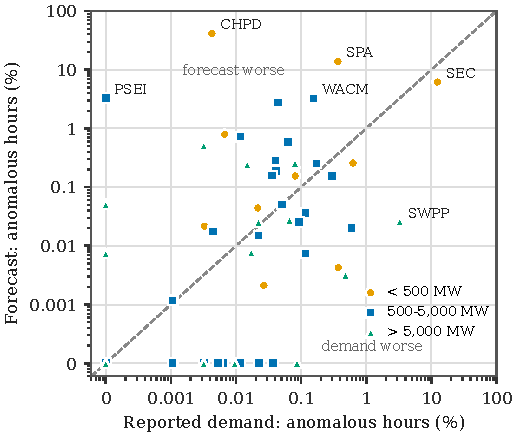
\includegraphics[width=\columnwidth]{fig_rates.pdf}
\caption{Share of hours in the shared classes (NONPOS, OVER, SPIKE, FLAT) for each BA, reported demand against forecast. Zero is plotted at the left and bottom edges. The dashed line marks equal rates.}
\label{fig:rates}
\end{figure}

\subsection{EIA's adjusted demand}
EIA changed a reported value in \res{eiaValTotal} BA-hours and filled \res{eiaFillTotal} empty cells. Of the changed values, \res{eiaValFlagged}\% are hours our screen flags. EIA's changes are therefore almost a subset of the screen. Agreement on gross outliers is expected, since both target values far from the weekly level; the informative part is what EIA leaves unchanged. Its changes cover only part of the screen (Table~\ref{tab:eia}):
\begin{itemize}
\item EIA changed nearly all gross outliers;
\item it changed \res{eiaPctNoSecNonpos}\% of non-positive values outside SEC, whose many zeros dominate that class;
\item it changed \res{eiaPctSpike}\% of spikes;
\item it changed none of the flat runs.
\end{itemize}
Without SEC, EIA changed \res{eiaNoSec}\% of the hours our screen flags.

The adjusted series also keeps errors of its own. In \res{adjAboveScr} BA-years the adjusted annual peak exceeds the peak of screened demand by more than 1\%, and in \res{adjAboveScrTen} by more than 10\%. PJM in 2020 is an example. Its reported annual peak is \res{pjmRepTwenty}~MW, EIA's adjusted peak \res{pjmAdjTwenty}~MW and our screened peak \res{pjmScrTwenty}~MW. All three are recording errors: PJM's adjusted peaks in 2019 and 2021 are \res{pjmAdjNineteen} and \res{pjmAdjTwentyOne}~MW, and even the screened 2020 value exceeds both by \res{pjmScrAboveNbr}\%. EIA corrected some of PJM's erroneous hours in 2020 but not others, and errors below twice the weekly median escape both EIA's adjustment and our screen. EIA does not adjust the forecast series at all.

\begin{table}[t]
\caption{Demand hours flagged by the screen, by class, and the share that EIA's adjusted demand changed}
\label{tab:eia}
\centering
\begin{tabular}{lrrr}
\toprule
Class & Flagged hours & EIA changed (\%) & without SEC (\%) \\
\midrule
NONPOS & \res{eiaNNonpos} & \res{eiaPctNonpos} & \res{eiaPctNoSecNonpos} \\
OVER & \res{eiaNOver} & \res{eiaPctOver} & \res{eiaPctNoSecOver} \\
SPIKE & \res{eiaNSpike} & \res{eiaPctSpike} & \res{eiaPctNoSecSpike} \\
FLAT & \res{eiaNFlat} & \res{eiaPctFlat} & \res{eiaPctNoSecFlat} \\
\bottomrule
\end{tabular}
\end{table}

\subsection{Effect on forecast accuracy}
H2 was supported. Screening changed the annual MAPE by more than 10\% in \res{hTwoK} of \res{hTwoN} BA-years (\res{hTwoShare}\%; interval \res{hTwoLo}--\res{hTwoHi}\%). These BA-years came from \res{hTwoBas} of the \res{hTwoBasOf} BAs.

The 10\% threshold is close to the median year-to-year change of a BA's screened MAPE (\res{yoyMed}\%; interquartile range \res{yoyLo}--\res{yoyHi}\%). In \res{hTwoBelowPp} of the \res{hTwoK} cases the change is below one percentage point (Section~\ref{sec:robust} gives absolute changes). The larger effects matter more: the change exceeded 50\% in \res{hTwoFifty} BA-years and 100\% in \res{hTwoHundred} (Fig.~\ref{fig:effects}a). The extreme case is \res{worstMapeBa} in \res{worstMapeYear}, with a raw MAPE of \res{worstMapeRaw}\% against \res{worstMapeScr}\% after screening.

The pre-specified screened MAPE removes SHIFT months. For \res{nDropped} BA-years (\res{hTwoDropped}) every month was flagged, so they have no screened MAPE. Realigning SHIFT months instead of removing them (exploratory) keeps all \res{hTwoRealN} BA-years and gives \res{hTwoRealShare}\% (\res{hTwoRealLo}--\res{hTwoRealHi}\%).

Rankings of BAs by MAPE move less than the levels. Kendall's $\tau$ \cite{kendall1945ties} between the raw and screened rankings ranged from \res{tauMin} (\res{tauMinYear}) to \res{tauMax} across years.

\begin{figure}[t]
\centering
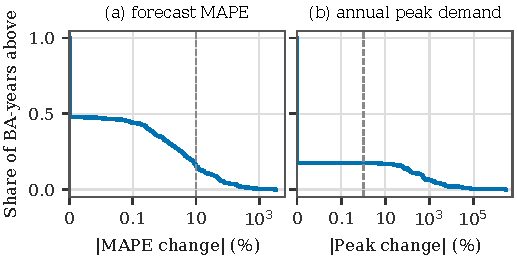
\includegraphics[width=\columnwidth]{fig_effects.pdf}
\caption{Share of BA-years whose (a) annual forecast MAPE changes by more than $x$ when anomalous hours are removed, and (b) annual peak from reported demand differs from the EIA-adjusted peak by more than $x$. Dashed lines: the H2 (10\%) and H3 (1\%) thresholds, with the share at each. BA-years with no change lie off the logarithmic axis.}
\label{fig:effects}
\end{figure}

\subsection{Effect on the annual peak}
H3 was supported. The reported annual peak differed from the adjusted one by more than 1\% in \res{hThreeK} of \res{hThreeN} BA-years (\res{hThreeShare}\%; interval \res{hThreeLo}--\res{hThreeHi}\%), from \res{hThreeBas} BAs. The reported peak was the larger one in \res{hThreeRepHigher} cases. The ratio of reported to adjusted peak was:
\begin{itemize}
\item above two in \res{ratioOverTwo} BA-years;
\item between 1.5 and 2 in \res{ratioMid};
\item between 1.01 and 1.5 in \res{ratioSmall}.
\end{itemize}
These are gross errors that any sanity check would catch. The annual maximum is the statistic most exposed to them, and an analyst who takes it from the reported column inherits them. The most extreme is PJM in \res{pjmSentinelYear}: a reported hourly demand of $\res{pjmSentinelGw}\times10^{9}$~MW against an adjusted peak of \res{pjmTrueGw}~GW (Fig.~\ref{fig:effects}b). Because the adjusted series keeps errors of its own, H3 is a lower bound.

The pre-specified measure of peak-day exposure ranks days by reported daily maximum demand. In \res{topK} of \res{topN} BA-years (\res{topShare}\%), at least one anomalous hour fell on a day among the year's top 5\%. This measure is partly circular: an upward spike lifts its own day into the top 5\%, and SHIFT months count as anomalous throughout. Ranking days by adjusted demand and leaving SHIFT out (exploratory) gives \res{topTwoShare}\% (\res{topTwoLo}--\res{topTwoHi}\%).

\subsection{Robustness (exploratory)}\label{sec:robust}
The checks of Amendment~2 are summarised here and in Table~\ref{tab:robust}.

\emph{H1.} With the forecast's reference built from the forecast itself, the forecast's shared rate exceeded demand's in \res{hOneOwnPos} of \res{hOneOwnN} BAs ($p\res{hOneOwnP}$). Without forecast flags at hours of anomalous demand, it did so in \res{hOneNdaPos} of \res{hOneNdaN} ($p\res{hOneNdaP}$). The demand-based reference does not explain the H1 result. H1 depends only on the SPIKE and FLAT settings (\res{gridNdistinct} combinations), and across them the forecast's rate was the higher one in \res{gridHOnePosLo} to \res{gridHOnePosHi} BAs. Only the loosest combination, SPIKE bounds $(\res{gridMinPSpikeHi}, \res{gridMinPSpikeLo})$ with FLAT runs of \res{gridMinPFlat} hours, gave a majority with $p<0.05$ (\res{gridMinPPos} of \res{gridMinPN}, $p\res{gridMinPP}$, not adjusted for the \res{gridNdistinct} combinations). In most BAs the forecast thus has more borderline flags than demand (mild deviations and short flat runs), but not more errors at the pre-specified bounds.

\emph{H2.} SHIFT is defined by an improvement in the forecast's fit, so removing SHIFT months could inflate H2 by construction. Keeping them as published gives \res{hTwoNsShare}\% (\res{hTwoNsK} of \res{hTwoNsN} BA-years). Across the \res{gridN} threshold settings, H2 ranged from \res{gridHTwoLo}\% to \res{gridHTwoHi}\%, and from \res{gridNsLo}\% to \res{gridNsHi}\% with SHIFT months kept, so it stayed above its 10\% threshold throughout. The COPY run length changed no result. In absolute terms, \res{hTwoAbsShare}\% of BA-years changed by at least one percentage point. Among the \res{hTwoK} BA-years above 10\%, the median change was \res{hTwoAbsMedHits} points (interquartile range \res{hTwoAbsQlo}--\res{hTwoAbsQhi}).

\emph{H3.} H3 does not use the screen. Every non-zero difference between reported and adjusted peaks exceeded \res{hThreeMinDiff}\%, so the share is the same at any threshold below that and falls only to \res{hThreeTenPct}\% at 10\%. H3 rests on gross errors. If differences in which the reported peak is more than twice the adjusted one are not counted, the share is \res{hThreeNoGross}\% (\res{hThreeNoGrossK} BA-years), below the 5\% threshold. H3 therefore measures exposure to errors that are easy to catch, not the difficulty of catching them.

\emph{Intervals.} Resampling whole BAs widens the intervals. Their lower bounds stay above the H2 and H3 thresholds for the pre-specified measures, but not for H2 with SHIFT months kept (\res{hTwoNsClLo}\%).

\emph{Extreme events.} Of the \res{evUriHours} BA-hours of Winter Storm Uri in ERCO, SWPP and MISO, the screen flagged \res{evUriDem} demand and \res{evUriFc} forecast hours. Of the \res{evElliottHours} BA-hours of Elliott in PJM, TVA and DUK, it flagged \res{evElliottDem} demand and \res{evElliottFcShared} forecast hours in the shared classes; PJM's forecast hours lay in SHIFT months (\res{evElliottFcShift} hours). The wide bounds did not mistake these extremes for errors, but the precision and recall of each class remain unknown.

\begin{table}[t]
\caption{Exploratory robustness of H2 and H3: share of BA-years (\%), with 95\% intervals that treat BA-years as independent or resample whole BAs}
\label{tab:robust}
\centering
\setlength{\tabcolsep}{3.5pt}
\begin{tabular}{lrrr}
\toprule
Measure & Share & Independent & BA bootstrap \\
\midrule
H2: MAPE change $>$10\% & \res{hTwoShare} & \res{hTwoLo}--\res{hTwoHi} & \res{hTwoClLo}--\res{hTwoClHi} \\
\quad SHIFT months realigned & \res{hTwoRealShare} & \res{hTwoRealLo}--\res{hTwoRealHi} & \res{hTwoRealClLo}--\res{hTwoRealClHi} \\
\quad SHIFT months kept & \res{hTwoNsShare} & -- & \res{hTwoNsClLo}--\res{hTwoNsClHi} \\
\quad \res{gridN} threshold settings & \res{gridHTwoLo}--\res{gridHTwoHi} & -- & -- \\
\quad same, SHIFT months kept & \res{gridNsLo}--\res{gridNsHi} & -- & -- \\
MAPE change $\ge$1 point & \res{hTwoAbsShare} & -- & \res{hTwoAbsClLo}--\res{hTwoAbsClHi} \\
\quad \res{gridN} threshold settings & \res{gridAbsLo}--\res{gridAbsHi} & -- & -- \\
H3: peak difference $>$1\% & \res{hThreeShare} & \res{hThreeLo}--\res{hThreeHi} & \res{hThreeClLo}--\res{hThreeClHi} \\
\quad difference $>$5\% & \res{hThreeFivePct} & -- & -- \\
\quad difference $>$10\% & \res{hThreeTenPct} & -- & -- \\
\quad reported $\le2\times$ adjusted & \res{hThreeNoGross} & -- & -- \\
\bottomrule
\end{tabular}
\end{table}

\subsection{Timestamp offsets (exploratory)}\label{sec:offsets}
The SHIFT class flagged months in \res{baFcShift} BAs. To see what lies behind them, we recomputed the MAPE month by month with the forecast shifted by $-3$ to $3$ hours, after removing gross errors (Fig.~\ref{fig:lag}, Table~\ref{tab:lag}).

From \res{firstPjm} onward, PJM's forecast row one hour \emph{earlier} matches demand best, in every one of \res{monthsPjm} months. The forecast is therefore stamped one hour early relative to demand, and delaying it by one hour realigns the two. The offset appears in all calendar months, both with and without daylight saving time, so it is a fixed relabelling, not a DST error. Realigning it lowers PJM's annual MAPE from \res{pjmMapeZero}\% to \res{pjmMapeBest}\%, which is PJM's level in 2016 to 2018 (\res{pjmMapePre}\%). A third of PJM's apparent error since 2019 thus comes from the offset. The same offset is reported in an erratum to the scorecard note \cite{guerrafilho2026scorecard}; our scan confirms it month by month and rules out DST as its cause.

The monthly diagnostic is symmetric. A demand series stamped one hour late would fit equally well, and would affect every study of PJM demand built on these files since 2019. PJM's official summer coincident peaks \cite{pjm5cp} decide between the two (exploratory). On the \res{cpN} official peak days of 2022 to 2026, EIA-930 reported demand peaks at PJM's official hour on \res{cpDem} days and within one hour on \res{cpDemWithin}, and its value at that hour is within \res{cpDemMwDev}\% of PJM's published peak load. The forecast as published peaks at the official hour on only \res{cpFc} days and earlier on \res{cpFcBefore} (mean difference \res{cpFcMean} hours). Delayed by one hour, it peaks at the official hour on \res{cpFcDel} days (mean \res{cpFcDelMean} hours); a day-ahead forecast need not peak at the actual hour, but it should not lead it systematically. Demand is therefore stamped correctly, and the forecast carries the offset. Since February 2019 the offset is present in \res{pjmStdMinus} of \res{pjmStdMonths} winter months (December to February, standard time) and \res{pjmDstMinus} of \res{pjmDstMonths} summer months (June to August, daylight time). The note \cite{guerrafilho2026scorecard} reports the same attribution from PJM's own load and forecast data.

Three other BAs show offsets:
\begin{itemize}
\item CISO in January to August 2016 and from July 2022 to November 2025. After realignment its error stays well above its earlier level, so the offset is not CISO's only problem. The note \cite{guerrafilho2026scorecard} traces the later offset to CISO's demand column, using CAISO's own data, and reports a real rise in CAISO's forecast error. We have not checked this.
\item AZPS, intermittently from \res{firstAzps}, by one or two hours. AZPS does not observe DST, so a mix-up between standard and prevailing time is a candidate.
\item SC, by $+1$ hour from \res{firstSc}.
\end{itemize}
Outside PJM we have no independent check, so for CISO in 2016, AZPS and SC it is open which series moved.

\begin{figure}[t]
\centering
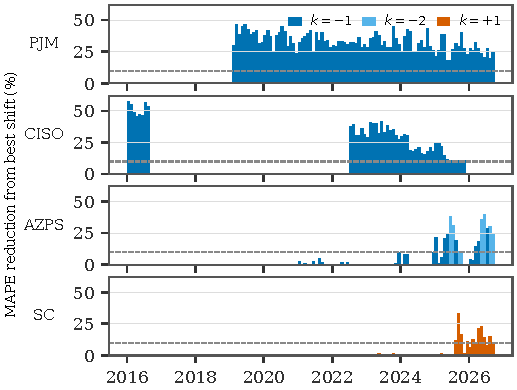
\includegraphics[width=\columnwidth]{fig_lag.pdf}
\caption{Monthly reduction in forecast MAPE from the best shift $k$ (forecast at $t+k$ paired with demand at $t$), for the four BAs with offsets; zero when the best shift is $k=0$. Dashed line: 10\%.}
\label{fig:lag}
\end{figure}

\begin{table}[t]
\caption{BA-years in which shifting the forecast lowers annual MAPE by at least 10\% (exploratory). MAPE (\%) averaged over the listed years.}
\label{tab:lag}
\centering
\setlength{\tabcolsep}{4pt}
\begin{tabular}{llrrr}
\toprule
BA & Years & Shift $k$ & MAPE, $k{=}0$ & MAPE, best $k$ \\
\midrule
\csname @@input\endcsname tab_lag.tex
\bottomrule
\end{tabular}
\end{table}

\section{Discussion}

The errors are rare in the typical hour but common enough in the typical analysis. A single sentinel can become a BA's annual peak, and percentage measures amplify a few bad hours \cite{hyndman2006another}. A sample check of the files shows clean data, while a sizeable minority of BA-years give wrong peaks or distorted accuracy.

We recommend four steps for users of the files:
\begin{enumerate}
\item Do not assume EIA's adjusted demand is clean. It fixes gross outliers and fills gaps but keeps spikes and flat runs, so screen it as well.
\item Screen the forecast series, which EIA does not adjust.
\item Check the alignment of forecast and demand per BA and month before comparing forecasts across BAs. The MAPE at shifts of $\pm1$ hour finds the offsets in Fig.~\ref{fig:lag}.
\item Report accuracy with and without screening, and prefer rankings or robust measures when screening changes the levels.
\end{enumerate}
For EIA, documenting each BA's time convention, flagging the values it adjusts and publishing an adjusted forecast column would remove most of these problems at the source.

\subsection*{Limitations}
\begin{itemize}
\item The thresholds are wide by design and miss errors within $[0.3, 2]$ times the weekly median, so the rates are lower bounds.
\item We have no hand-labelled sample, so the precision and recall of each class are unknown. The extreme-event check covers only two storms.
\item EIA's adjusted values are a reference, not ground truth.
\item The files are revised over time. Our results describe the November 2026 vintage.
\item BA-years are not independent. The pre-specified intervals for H2 and H3 are optimistic; the BA-cluster bootstrap is exploratory.
\item The offset analysis is exploratory. Only PJM's attribution is checked against official data, and the causes are unknown.
\item The pre-specified comparison with the cleaned data of Ruggles et al.\ was not carried out. Those data cover 2015--2019 from an older vintage.
\end{itemize}

\section{Conclusion}
Recording errors in EIA-930 are rare in the typical hour but common in the typical analysis. Removing them changes a BA-year's forecast MAPE by more than 10\% in about one case in six, and the reported annual peak is grossly inflated in about one case in six. EIA's adjusted demand fixes some of these errors but not all, and none in the forecast. A one-hour offset in PJM's forecast, also reported in \cite{guerrafilho2026scorecard} and placed in the forecast by PJM's official peak hours, has inflated PJM's apparent forecast error by half since 2019. Screening both series and checking their alignment are cheap steps that should precede any forecast evaluation on these data.

\section*{Data and code availability}
The analysis plan with its commit history and amendments, the code and the result files are available at \url{\repoURL}. The data are the public EIA-930 files. PJM's reports are not redistributed; their URLs and SHA-256 hashes are in the code.

\section*{Acknowledgment}
The author used Claude Opus 5.5 (Anthropic; model identifier claude-opus-5-5) to help write analysis code and draft and edit the text. The author checked the code, the results and the text and takes full responsibility for the content.

\bibliographystyle{IEEEtran}
\bibliography{refs}

\end{document}
